\documentclass[addpoints]{exam}
\usepackage[utf8]{inputenc}
\usepackage[portuguese]{babel}
\usepackage[LGRgreek]{mathastext}
\usepackage{graphicx,graphics}

\footer{}{\thepage}{}
 
\pointpoints{ponto}{pontos}
\bonuspointpoints{ponto extra}{pontos extra}
 
\totalformat{Pregunta \thequestion: \totalpoints pontos}
 
\chqword{Pregunta}
\chpgword{Página}
\chpword{Pontos}
\chbpword{Pontos extra}
\chsword{Pontos obtidos}
\chtword{Total}

\hqword{Questão}
\hpgword{Página}
\hpword{Pontos}
\hsword{Pontos obtidos}
\htword{Total}

 
\begin{document}
 
\begin{center}
Eletrônica Básica II – EE640 U - Lista de Exercícios 2
\end{center}
 
\vspace{5mm}
 
\makebox[0.72\textwidth]{Nome: \enspace\hrulefill}
\hfill
\makebox[0.2\textwidth]{RA: \enspace\hrulefill}

\begin{center}
A lista deve ser entregue até dia \textbf{01-01-1968}
\end{center}

\hspace{2mm}

\begin{center}
\gradetable[h][questions]
\end{center}

\hspace{2mm}

\begin{questions}

\question A Figura apresenta um amplificador \textit{cascode}. O projeto prevê uma impedância de saída ($R_{OUT}$) de 1200 $k\Omega$. A corrente de polarização é 1 mA. 

\begin{minipage}[m]{0.7\textwidth}
\begin{parts}
 \part[2] Considerando que os transistores são casados e possuem $\vert V_A \vert = 80$ V, $k'_n = 10$ $\mu A/V^2$, calcule $(W/L)_1$ e $(W/L)_2$.
 \part[1] Calcule o ganho de tensão do amplificador \textit{cascode}.
 \part[1] Com os valores obtidos, apresente o modelo de pequenos sinais.
 \part[1] Com o \textbf{modelo de pequenos sinais}, calcule $v_O/v_I$ para $R_{L1} = 100$ $k\Omega$ e $R_{L2} = 1$ $M\Omega$.
\end{parts}
\end{minipage}
\hspace{5mm}
\begin{minipage}[m]{0.2\textwidth}
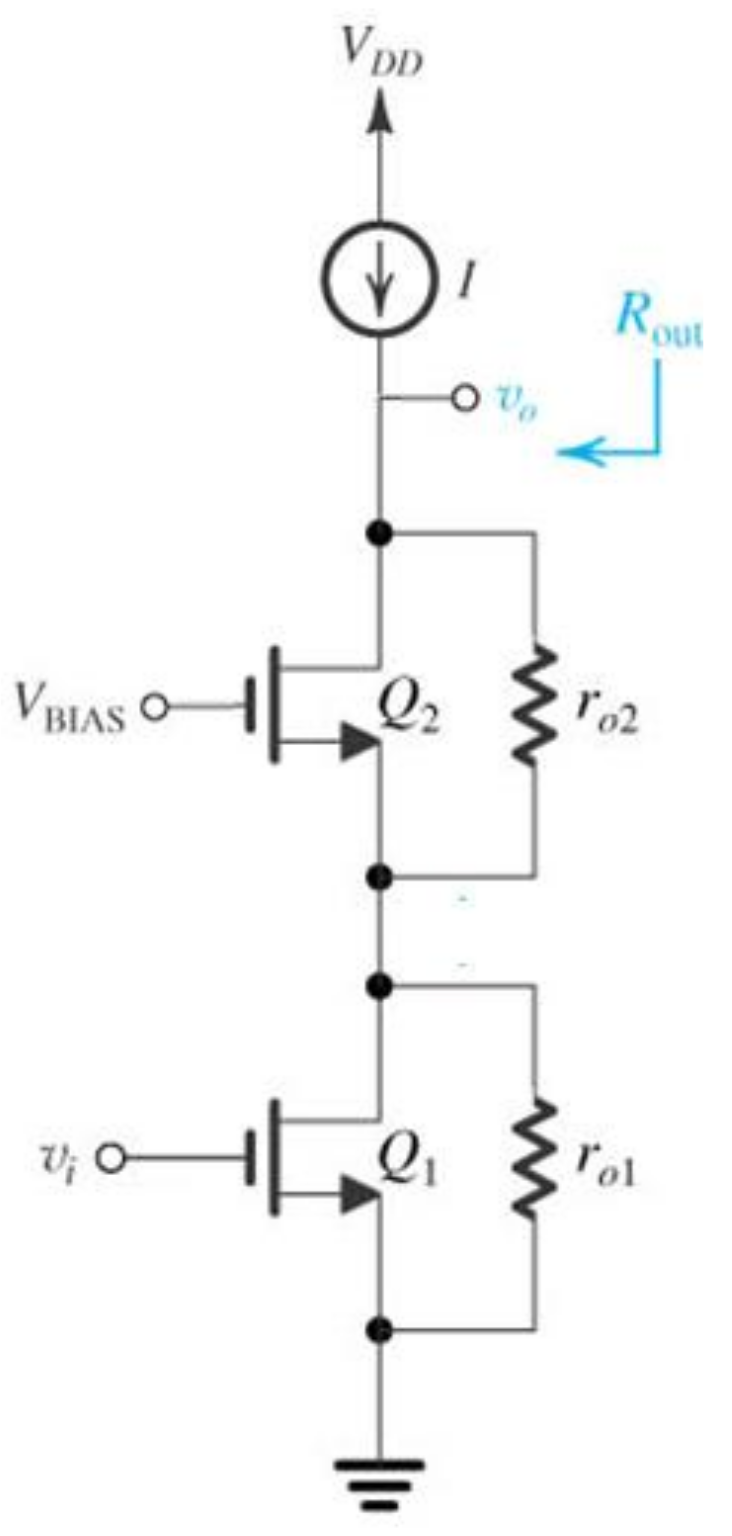
\includegraphics[width=\textwidth]{imagens/1.png}
\end{minipage}

\question[4] Deseja-se projetar o espelho de corrente da Figura para uma corrente de saída de 500 $\mu A$. Deve-se garantir que a tensão de saída opere entre a faixa de 500 mV até no máximo $V_{DD}$ V e que a variação do valor nominal de $I_O$ para esta faixa esteja limitada a 2 \%. Considere que o valor da corrente de saída fora obtido quando $V_O = V_{GS}$. Encontre o valor de R e as dimensões dos transistores $Q_1$ e $Q_2$.

\begin{minipage}[t]{0.3\textwidth}
\begin{itemize}
    \item $k'_n = 400$ $\mu A/V^2$
    \item $V'_A = 100$ $V/\mu m$
    \item $V_t = 0,5$ V
    \item $V_{DD} = 2,5$ V
\end{itemize}
\end{minipage}
\hspace{5mm}
\begin{minipage}[m]{0.4\textwidth}
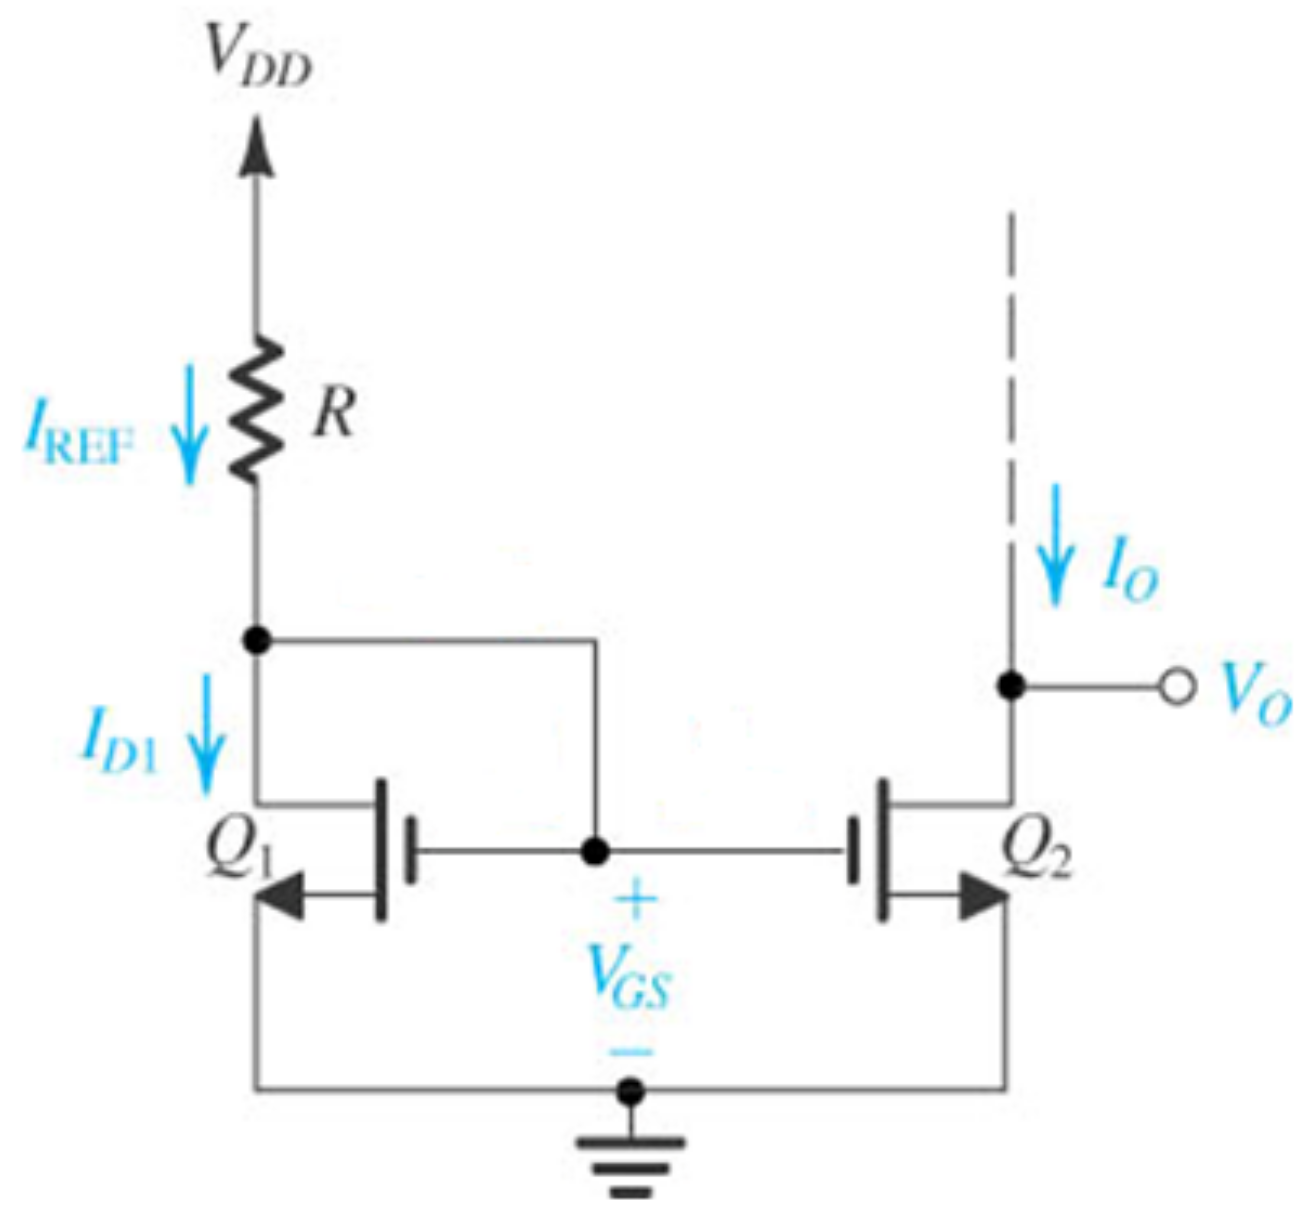
\includegraphics[width=\textwidth]{imagens/2.png}
\end{minipage}

\question Um projetista utilizou uma fonte de corrente com impedância de saída ($R_{SS}$) e uma fonte de sinal único ($V_{CM}$) para polarizar os transistores do amplificador diferencial da Figura. A fonte de corrente estabelece uma corrente de 1 mA. Os transistores $Q_1$ e $Q_2$ tem $V_t = 0,8$ V, $k'_n = 1$ $mA/V^2$, W/L = 5, $\lambda = 0$, $V_{DD} = 15$ V e $V_{SS} = 0$ V. Considere uma queda de 1 V na fonte de corrente, ou seja, $\vert V_{CS} \vert = 1$ V.

\begin{parts}
 \part[1] Qual o valor de $V_{CM}$ que garante o funcionamento do circuito como amplificador?
 \part[1] Se o valor de $R_D$ variar entre 3 $k\Omega$ e 10 $k\Omega$ (potenciômetro), qual a variação ($\Delta A_V$) do ganho diferencial (saída diferencial)?
 \part[1] Qual a tensão \textit{cc} nos drenos dos transistores para $R_D = 8$ $k\Omega$
 \part Determine o ganho de modo comum (saída única) para $R_D = 8$ $k\Omega$ levando em consideração o valor de $g_m$.
 \label{2d}
 \part[1] Calcule o valorde CMMRu em dB usando o valor do item \ref{2d}.
 \part[1] Calcule o valor de CMMRd usando o valor do item \ref{2d}.
 \part[1] Se a saída for diferencial e existir um erro de 1 \% entre as resistências de dreno, qual o valor de $\vert A_d \vert$, $\vert A_{cm} \vert$ e CMMRd? Considere $R_D = 8$ $k\Omega$.
\end{parts}

\begin{center}
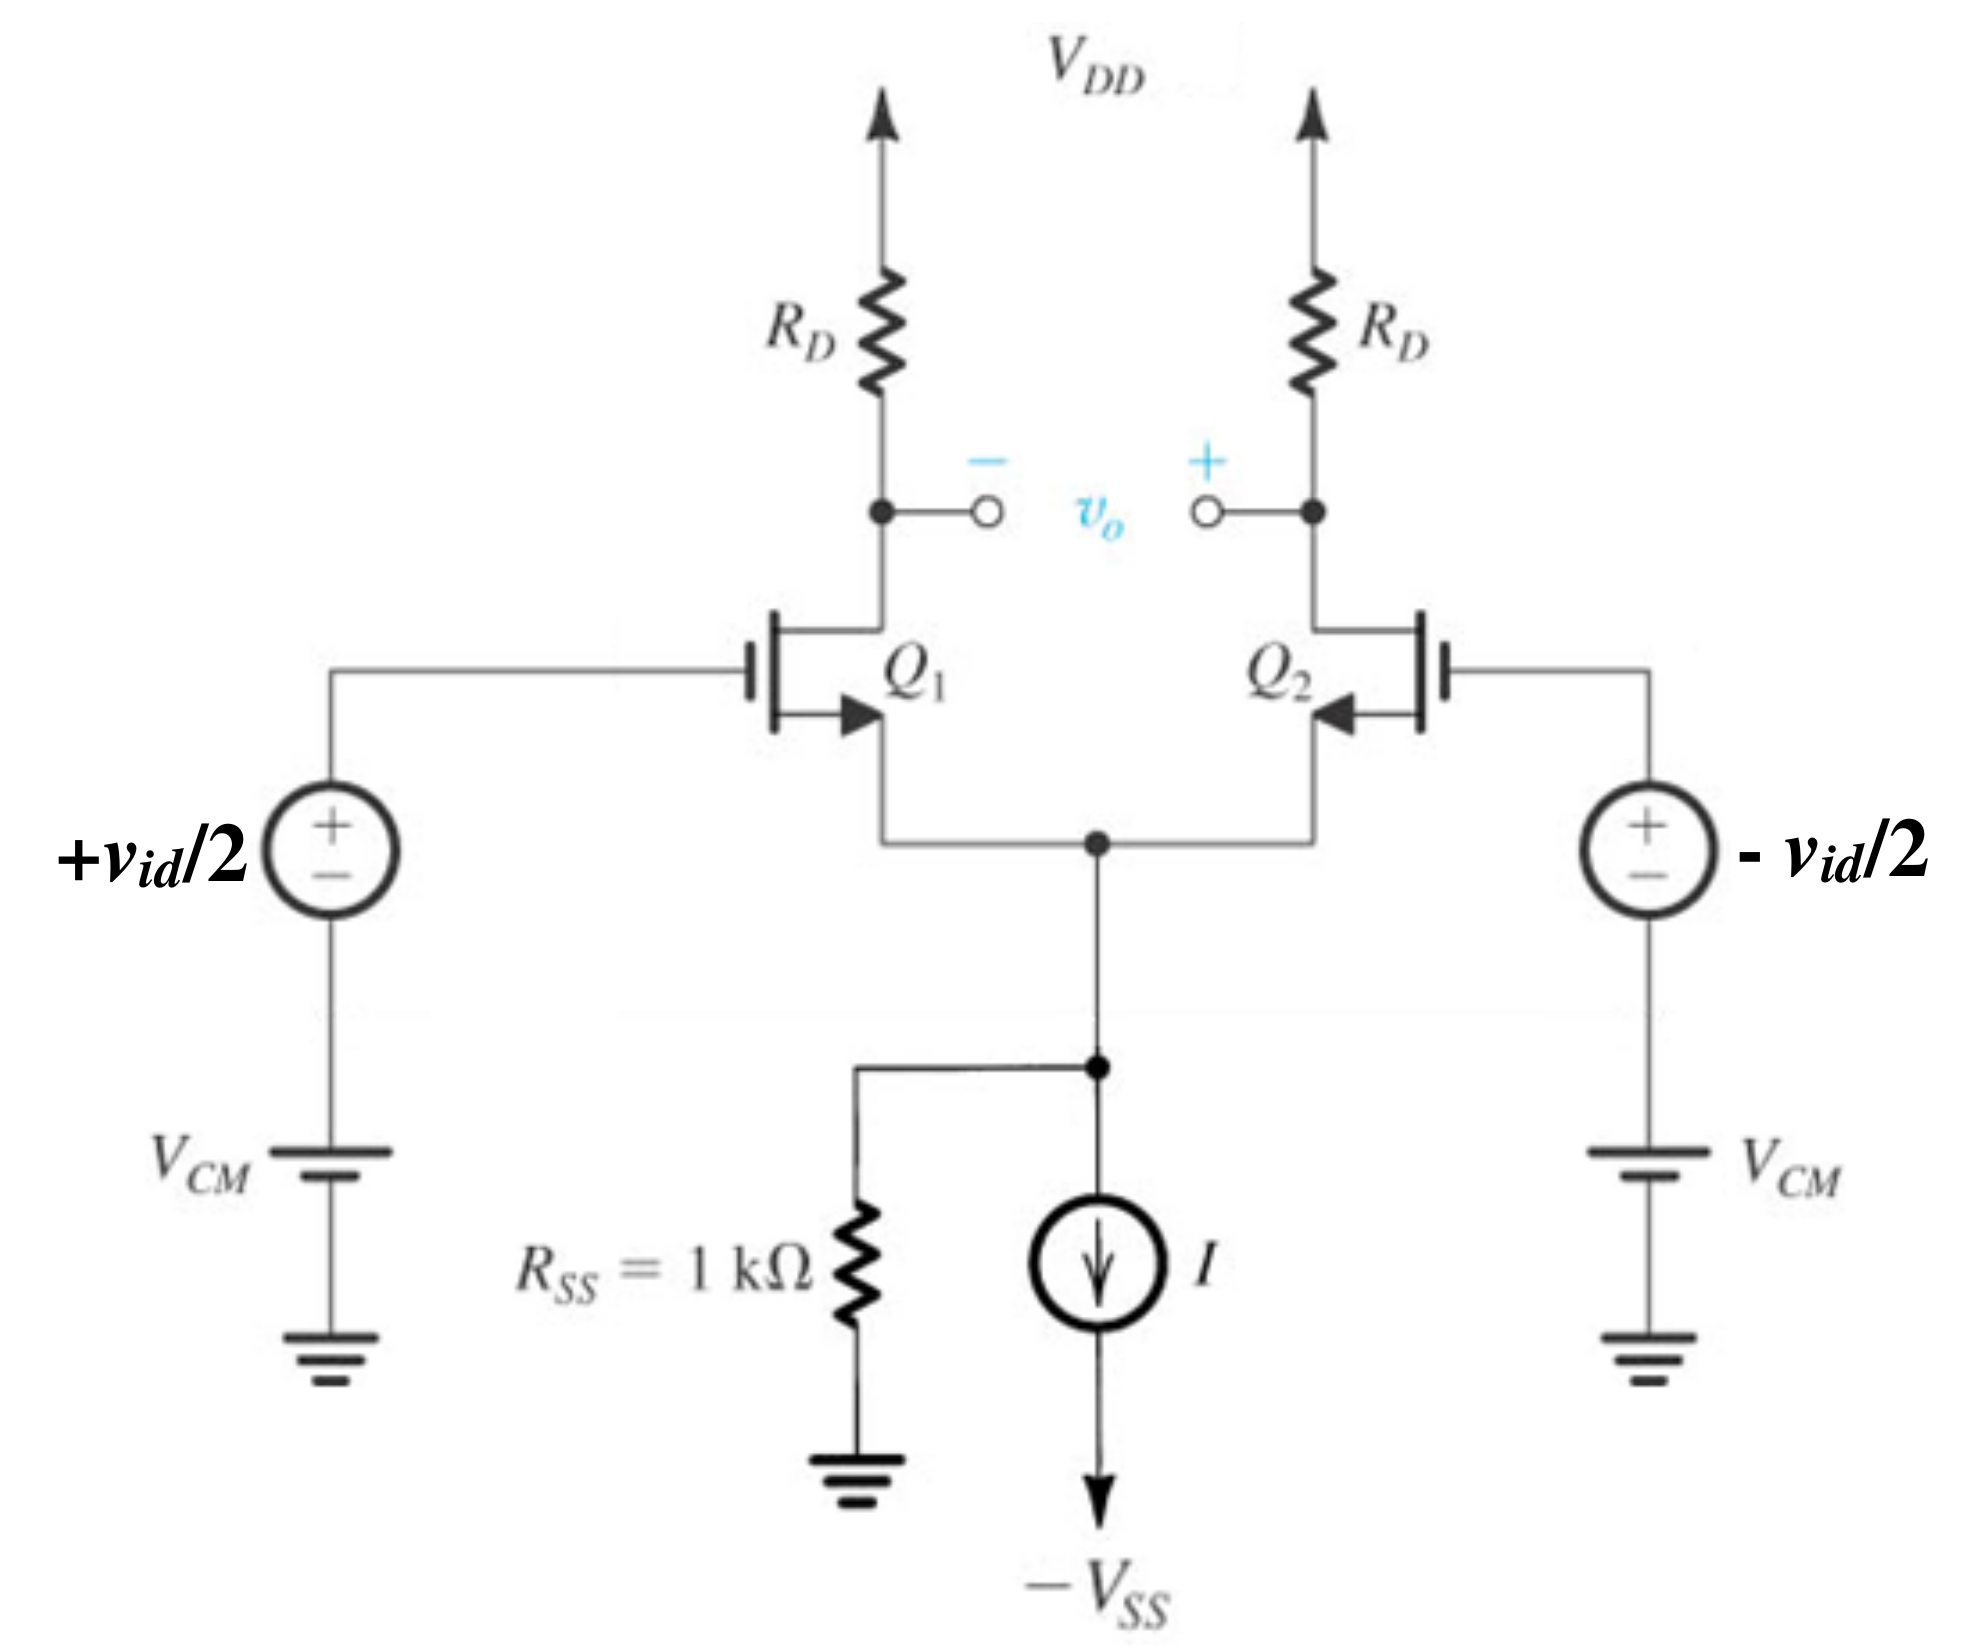
\includegraphics[width=0.55\textwidth]{imagens/3.png}
\end{center}

\question[2] Explique o funcionamento do amplificador do tipo ``Par Darlington''.

\question[1] Quais as limitações e qual a principal utilização do amplificador diferencial BJT?

\question[3] Projete o amplificador fonte comum da Figura para um ganho de tensão de 28 V/V e máxima potência dissipada de 4 mW. Use $(W/L)_1 = 20/0.25$, $\lambda_n = 0,15$ $V^{-1}$ e $\lambda_p = 0,25$ $V^{-1}$, $k'_n = 150$ $\mu A/V^2$ e $V_t = 0,5$ V.

\begin{center}
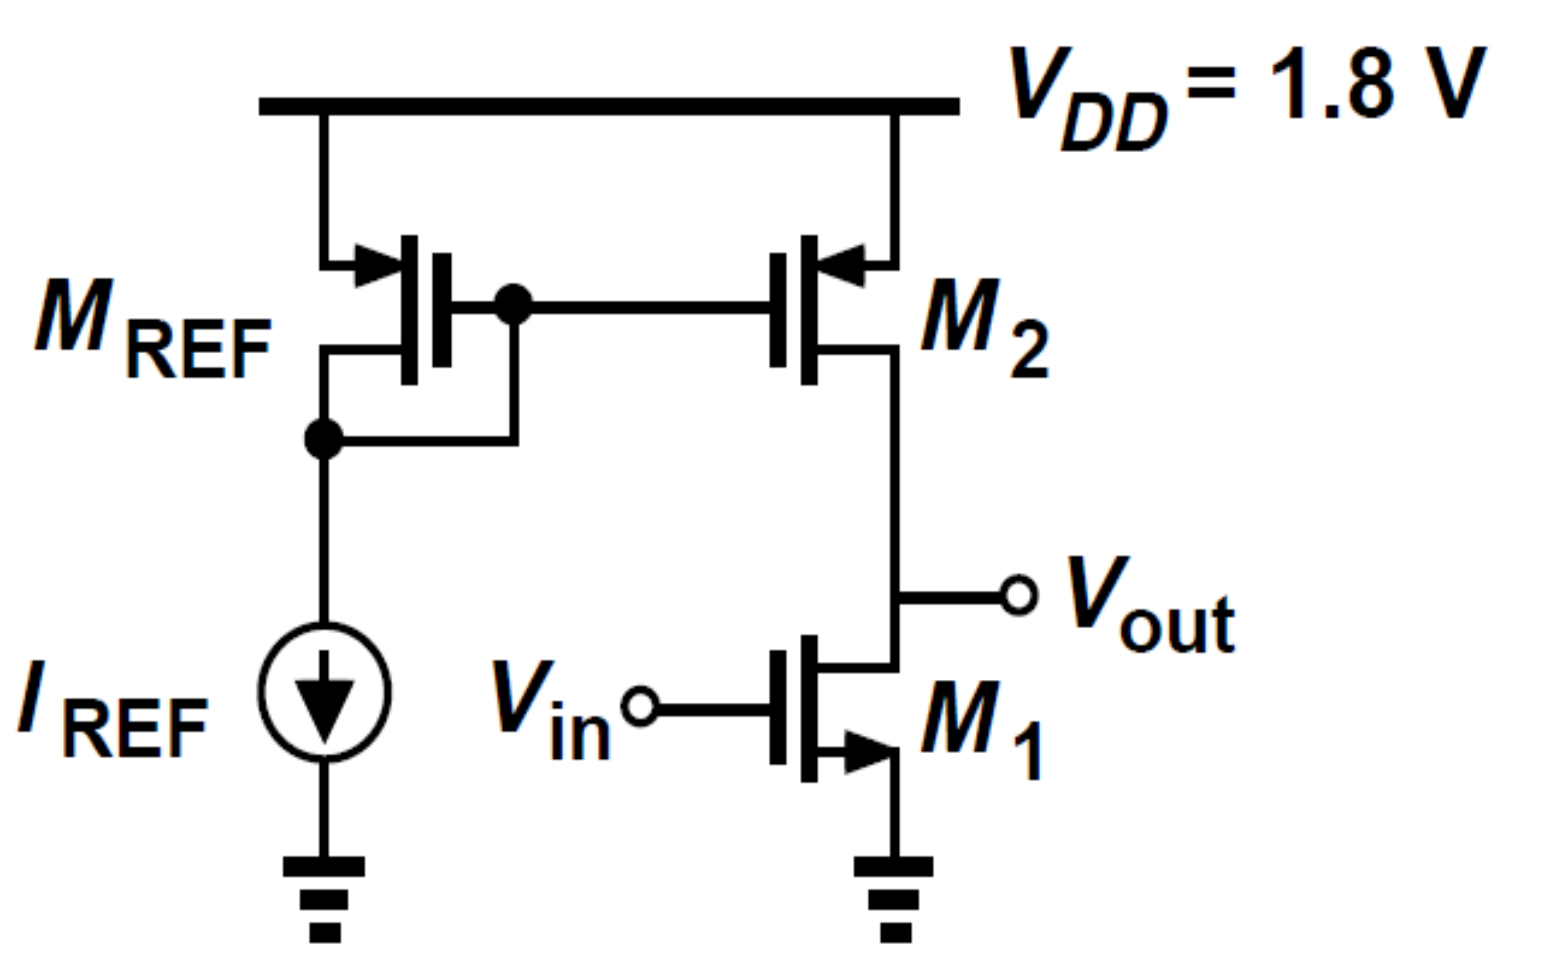
\includegraphics[width=0.4\textwidth]{imagens/4.png}
\end{center}

\end{questions}

\end{document}
